\documentclass{article}
\usepackage[utf8]{inputenc}
\usepackage{color}
\usepackage{xcolor}
\usepackage{pgfplots}
\usepackage{amsmath,amssymb}
\usepackage{graphicx}
\usepackage[hidelinks]{hyperref}
\pgfplotsset{compat=newest}
\setlength{\parindent}{0pt}
\title{Sentence Decomposition: Analyzing the problem}
\author{Simón Marín Giraldo}
\date{\today}
\begin{document}
	\begin{titlepage}
		\centering
		{\bfseries\LARGE Universidad EAFIT \par}
		\vspace{1cm}
		{\scshape\Large Departamento de Informática y Sistemas \par}
		\vspace{3cm}
		{\scshape\Huge Sentence Decomposition: Analyzing the problem \par}
		\vspace{3cm}
		{\itshape\Large Data Structures and Algorithms II \par}
		\vfill
		%{\Large Author: \par}
		{\Large Simón Marín Giraldo \par}
		{\Large Julián Ramírez Giraldo \par}
		{\Large May 2020 \par}
	\end{titlepage}
	%\maketitle
	\newpage
	\tableofcontents
	\newpage
	\section{Introduction}
	\subsection{Problem definition}
	We are given a String problem in which we are requested to
	minimize the cost of operations over sequences of characters.
	\\
	We receive a list of valid words and a sentence that can
	contain the accepted words from the list. This sentence
	contains each word from the list but their characters are
	mixed. Anyway, the order in which the mixed words appear
	is the same as the order of the words in the dictionary.
	\\
	\\
	\textbf{For example:}
	\\
	\\
	We have the sentence: \textbf{``neotowheret''}
	\\
	And we have the dictionary: \textbf{\{``one'', ``two'', ``three'', ``there''\}}
	\\
	Even if we have the sentence in disorder, the order of
	the dictionary is kept:
	\\
	\\
	The underlined part in the sentence:
	\begin{center}
		\textbf{``$\underline{\textbf{neo}}$towheret''}
		\\
	\end{center}
	Matches with the first word in the dictionary:
	\begin{center}
		\textbf{\{``$\underline{\textbf{one}}$'', ``two'', ``three'', ``there''\}}
		\\
		\vspace{1pt}
	\end{center}
	Then we have the second visible valid word:
	\begin{center}
		\textbf{``neo$\underline{\textbf{tow}}$heret''}
		\\
	\end{center}
	It matches with the second word in the dictionary:
	\begin{center}
		\textbf{\{``one'', ``$\underline{\textbf{two}}$'', ``three'', ``there''\}}
		\\
	\end{center}
	Let's now take a look at the two last elements in
	our dictionary:
	\begin{center}
		\textbf{\{``one'', ``two'', ``$\underline{\textbf{three}}$'', ``$\underline{\textbf{there}}$''\}}
		\\
	\end{center}
	As we can notice, with the last five characters in
	our sentence, we can build any of the last two words
	in the dictionary.
	\\
	\begin{center}
		\textbf{``neotow$\underline{\textbf{heret}}$''}
		\\
	\end{center}
	With the following definitions and the solution explanation,
	we will determine how to optimally minimize the \emph{\textbf{cost}} of
	transformation and solve the problem.
	%Llenar esta parte con la definición del problema
	\subsubsection{Concepts}
	\begin{itemize}
		%\item \emph{\textbf{Word length}}: it is defined as the number
		%of character that a String has. We will have a word length set.
		\item \emph{\textbf{Cost}}: it is defined as the number of
		characters in which two given Strings differ.
		\\
		\\
		\textbf{For example:}
		\\
		\\
		Let's consider the following Strings:
		\begin{center}
			``neo''
			\\
			``one''
			\\
		\end{center}
		As explained in the previous definition, \emph{\textbf{cost}}
		is the number of character positions in which
		two Strings differ. In this case, the first
		character of the first String is ``n''. Now,
		let's look at the first character in the second
		String. It is ``o''. As ``n'' $\ne$ ``o'', we
		proceed to add 1 to the \emph{\textbf{cost}}.
		\\
		\\
		Now, let's take a look at the second character in
		each String. For the first String's second character
		we have ``e''. Now, for the second String's second
		character, we have ``n''. As ``e'' $\ne$ ``n'', we
		add 1 to the \emph{\textbf{cost}}. Now, the \emph{\textbf{cost}} has a value of 2
		because we have found two character positions in
		which both Strings differ.
		\\
		\\
		Finally, let's see the third and last character in
		both Strings. For the first String's third character
		we have ``o''. Now, for the second's String third
		character, we have ``e''. As ``o'' $\ne$ ``e'', we
		add 1 to the \emph{\textbf{cost}}. Now the total \emph{\textbf{cost}} has a value
		of 3 because we found three character positions in
		which both Strings differ.
		%Llenar esta parte con el ejemplo para costo
		
		\item \emph{\textbf{Anagram}}: Two words are anagrams when
		they both have the same length and the same quantity of each
		character.
		\\
		\\
		\textbf{For example:}
		\\
		\\
		Let's consider the following Strings:
		\begin{center}
			``three''
			\\
			``heret''
			\\
		\end{center}
		As explained in the previous definition, anagrams are words
		that have both the same length and the same quantity of each
		character.
		\\
		First of all, we need to make sure that both words have the same
		length:
		\begin{center}
			$|``three''| = 5$
			\\
			$|``heret''| = 5$
			\\
		\end{center}
		As we can see, both Strings have the same length.
		Now, we start counting the quantity of each character:
		\begin{center}
			$|``three''|_t = 1$
			\\
			$|``heret''|_t = 1$
			\\
		\end{center}
		As we can see, we have the same number of ``t'' characters
		in both Strings. We continue with all the other characters:
		\begin{center}
			$|``three''|_h = 1$
			\\
			$|``heret''|_h = 1$
			\\
			$|``three''|_r = 1$
			\\
			$|``heret''|_r = 1$
			\\
			$|``three''|_e = 2$
			\\
			$|``heret''|_e = 2$
			\\
		\end{center}
		As we can see, every character in ``three'' is present
		in ``heret'' in the same quantity.
		\\
		\\
		A more formal definition for anagrams would be:
		\\
		\\
		Let $\Sigma$ be an alphabet.
		\\
		Let $x, y$ be some words with $\Sigma$ symbols.
		\\
		Let $|x|_a$ be the total amount of a's in x
		i.e: $|aab|_a = 2, |aab|_c = 0$.
		\\
		\\
		Now, we can define
		\\
		A: $word \times word$ $\to$ $\{true, false\}$
		as a function such that:
		%\begin{center}
			\[
				A(x,y)=
			\begin{cases}
				true, & \text{if } |x| = |y| \text{ and } |x|_\delta = |y|_\delta, \forall_\delta \in \Sigma
				\\
				false, & \text{otherwise}
			\end{cases}
			\]
		%\end{center}
	\end{itemize}
	\subsection{Input}
	\begin{itemize}
		\item \emph{\textbf{Sentence: String}}: This parameter is
		a String which is going to be analyzed and compared with
		words in a dictionary.
		
		\item \emph{\textbf{Dictionary: String array}}: This
		parameter is the dictionary which will be used to
		analyze the sentence.
	\end{itemize}
	\subsection{Output}
	The program will return an integer that will represent the
	minimum total \emph{\textbf{cost}} that will be needed to turn the given
	sequence into a sequence with the accepted words which are
	specified in the dictionary. If there is no such possible
	transformation that will allow us to convert the given
	sequence into a sequence made from the accepted words,
	the result to be returned will be -1.
	\section{Solution and complexity analysis}
	Now, we are going to describe the coding solution given
	to this particular problem. We must take into account that
	this solution must work for every case for it to be a valid
	solution accepted by the online judge.
	\subsection{Determining anagrams}
	We previously defined what was an anagram and a method for
	finding them. Since we are concerned about optimizing the execution
	times and algorithmic complexity, we must have an optimal method
	to determine if two words are anagrams. Instead of counting each
	type of character in a word, checking with the next ones and comparing
	each character length, which has a complexity of:
	\[
	T(m)_1 = \underbrace{mk}_x + \underbrace{mk}_y
	\]
	\\
	\[
	O(m^2)
	\]
	\\
	Where $m$ is the length of the word and $k$ is the number of symbols in
	the alphabet $\Sigma$.
	\\
	\\
	The final Big-O notation for this operation will be: $O(m^2)$.
	\\
	We can optimize this by changing our anagrams method for a
	less complex one.
	%MODIFICAR LAS ECUACIONES DE AQUI PA ABAJO Y METERLES DOS VARIABLES
	\subsubsection{Optimizing the anagrams comparison}
	The new challenge is to optimize the method that determines if two
	words are anagrams or not.
	\\
	As we can see, we have the same length and the same letters in words
	for them to be anagrams. This gives us a clue for a criteria to determine
	whether they are anagrams or not.
	\\
	If we have the same characters in both Strings, we will have the same String
	if we sort both Strings. Then, we can compare them. If we have the same, then
	those Strings are anagrams. Now the issue is that comparing two Strings means
	$m$ operations, where $m$ is the length of the Strings. This is not a big
	issue as we finally have a $T(m)_2 < 2m$:
	\[
	T(m)_2 = \underbrace{m \times log(m)}_\text{from quicksorting String x} + \underbrace{m \times log(m)}_\text{from quicksorting String y} + \underbrace{m}_\text{from comparison}
	\]
	\[
	T(m)_2 = 2(m \times log(m)) + m
	\]
	\[
	O(m \times log(m))
	\]
	Where $m$ is the length of the String.
	\\
	\\
	Now, let's compare $O(m^2)$ and $O(m \times log(m))$:
	\\
	\begin{center}
		\textcolor{blue}{$O(m^2)$}
		\\
		\textcolor{red}{$O(m \times log(m))$}
		\\
		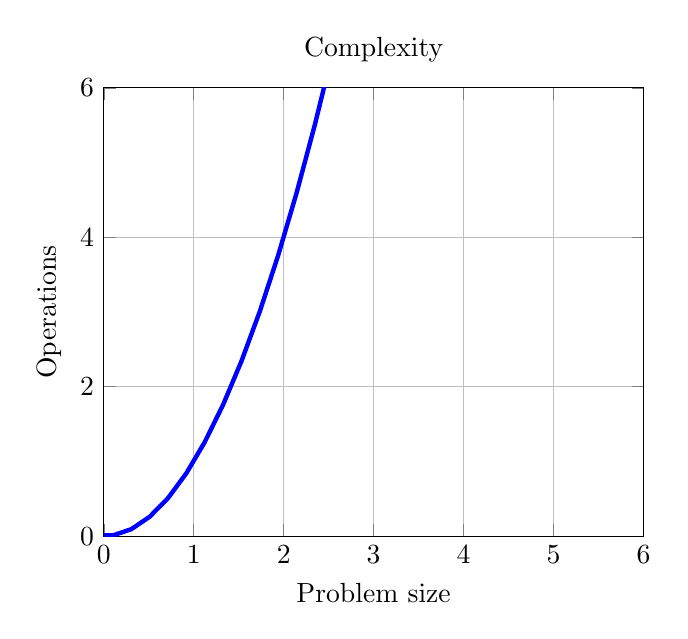
\begin{tikzpicture}
		\begin{axis}[xmin=0,xmax=6,ymin=0,ymax=6,samples=50,grid=major,xlabel={Problem size},ylabel={Operations},title={Complexity}]
		\addplot[blue, ultra thick](x,x*x);
		%\addplot[red, ultra thick](x,x*log10(\x));
		\end{axis}
		\end{tikzpicture}
	\end{center}
	As we can see in the graph above, the \textcolor{red}{$O(m \times log(m))$} curve grows
	slower than \textcolor{blue}{$O(m^2)$} curve.
	\\
	\\
	\textbf{Conclusion:} The best way to determine if some words are anagrams
	is by sorting and comparing them.
	\subsection{Preparing for dynamic programming}
	We are going to begin our algorithm adapting it to work
	with \textbf{dynamic programming}.
	\subsubsection{Copying the original sentence length}
	We start creating a length variable to copy in it the length
	of the initial sentence. We do this because the sentence will
	be altered during the further algorithm operations. This will
	take a constant number of operations of $1$.
	\[
	T(m, n, p)_\text{total} = \underbrace{1}_\text{from copying the length into a new variable}
	\]
	\subsubsection{Creating dynamic programming array}
	In this part, we are concerned about creating an array for
	memorization of operations answers, in order to reduce the
	complexity by avoiding the operation repetition. This will
	take a constant number of operations of $1$ that will be
	added to the total number of operations.
	\[
	T(m, n, p)_\text{total} = 1 +	\underbrace{1}_\text{from creating the dynamic programming array}
	\]
	\subsubsection{Filling dynamic programming array with max value}
	In order to identify the base cases and general cases, we need
	to fill our \textbf{dynamic programming} array with the value
	from \textbf{Integer.MAX\_VALUE}. This will take $n + 1$ operations
	which will be added to the total number of operations.
	\[
	T(m, n, p)_\text{total} = 1 + 1 + \underbrace{n + 1}_\text{from filling \textbf{dynamic programming} array with \textbf{Integer.MAX\_VALUE}}
	\]
	Where $n$ is the length of the sentence to be analyzed. In this case, we have
	to add $1$, which corresponds to the $\text{copied sentence length} + 1$.
	\\
	\\
	Now, we are going to assign the value $0$ to the first element
	in the \textbf{dynamic programming} array. This will take a
	constant number of operations of $1$ that will be added to the
	total number of operations.
	\[
	T(m, n, p)_\text{total} = 1 + 1 + n + 1 + \underbrace{1}_\text{from assigning 0 to the \textbf{dynamic programming} array in position 0}
	\]
	\subsection{Finding anagrams}
	\subsubsection{Determining iteration and general cases}
	Now, we are going to declare a loop which is going to
	iterate $n$ times (remember that $n$ is the sentence length). Nevertheless, this will not
	happen every time. We have to check first whether the position
	in the array in the current $i$ iteration value is less than
	\textbf{Integer.MAX\_VALUE}. As values inside the array will
	be changing, this verification will take 1 operation and as
	it will be done in every iteration.
	\[
	T(m, n, p)_\text{total} = 1 + 1 + n + 1 + 1 + [\underbrace{1}_\text{verification} \times \underbrace{n}_\text{iterations}]
	\]
	Then we have to do another conditional iteration inside the
	one above. This one will go through the words in the dictionary.
	This conditional iteration will happen only if \textbf{two conditions}
	are satisfied:
	\begin{itemize}
		\item The sum between the current $i$ iteration and the length of
		the current word in the dictionary is equal or less than the length
		of the sentence being analyzed. This is necessary because the problem
		definition will no have sense if any word in the dictionary is longer
		than the sentence. That sentence couldn't be formed. This will take
		$1$ operation for the addition and $1$ for comparing with the $length$.
		\[
		T(m, n, p)_\text{total} = 1 + 1 + n + 1 + 1 + \{1 \times n \times [\underbrace{1}_\text{addition} + \underbrace{1}_\text{comparison}]\}
		\] 
		Simplifying the expression we get:
		\[
		T(m, n, p)_\text{total} = 4 + n + \{n \times 2\}
		\]
		\item The current word in the dictionary and the subsequence being
		analyzed must be anagrams. If they are not, there wouldn't exist a
		transformation such that we can reach the target sequence with the
		characters in the current subsequence. This will take $m$ for the
		subsequence extraction steps. This will be inside the method for determining
		if two words are anagrams, which takes $2(m \times log(m)) + m$ steps.
		\[
		T(m, n, p)_\text{total} = 4 + n + \{n \times 2 \times [\underbrace{m}_\text{subsequence} \times \underbrace{(2(m \times log(m)) + m)}_\text{anagrams} \times \underbrace{p}_\text{dictionary size}]\}
		\] 
		%reemplazar end y begin con sus correspondencias en una nueva ecuacion
	\end{itemize}
	\vspace{2pt}
	
	\subsection{Cost operations and minimization}
	Now that we have determined the constraints for our iterations, we
	must solve the most important part of our problem which is determining
	and minimizing the cost to transform from one String to another. The
	following operations will be described assuming that the iteration
	constraints have been satisfied.
	\\
	\\
	What we have to do now is to memorize with \textbf{dynamic programming}.
	We are going to assign into the array positions, the minimum values
	of cost that solve our problem. This values are found with two constraints
	for each possible couple that can be minimized:
	\begin{itemize}
		\item In the current position, we start checking from left to right
		with the cost for transformation of the current subsequence into the
		dictionary word. This will take %ojo a este paso
		\item The latest infallible element plus the cost of the current word
		that is being analyzed. This will
		take $1 + m \times m$ operations.
		\begin{multline*}
		T(m, n, p)_\text{total} = 4 + n + \{n \times 2 \times [m \times (2(m \times log(m)) \\ + m) \times p \times (\underbrace{1}_\text{array access} + \underbrace{m}_\text{\emph{\textbf{cost}}} \times \underbrace{m}_\text{subsequence})]\}
		\end{multline*}
	\end{itemize}
	We are going to pick the minimum between this two. This will take $1$ operation
	from the comparison, plus the steps taken by both possibilities which have to be
	done to get the minimum
	\\
	Finally, we return the value in the length position because this one is
	the last one calculated, which contains the total, that has been growing
	from the previous minimum \textbf{\emph{cost}} values.
	%solution stuff
	\subsection{Final complexity}
	After solving the expression, we get a final asymptotic complexity of: $O(n \times m^2 \times log(m))$.
\end{document}